\section{Determinantes e Inversas}

Objetivos del Capítulo:

\begin{itemize}
\item
Estudiar la definición inductiva de los determinantes.

\item
Aprender las propiedades fundamentales de los determinantes.

\item
Relacionar la determinante de una matriz con la existencia de su inversa.

\end{itemize}

\subsection{Determinantes}
Como vimos en el m\'odulo anterior, una matriz de orden dos $A=(a_{ij})$ es invertible si y s\'olo si el n\'umero $a_{11}a_{22}-a_{12}a_{21}$ es distinto de cero, n\'umero que adem\'as nos permite encontrar la inversa de la matriz. Este n\'umero real puede definirse para matrices de cualquier orden y aparace en un gran n\'umero de \'areas de la matem\'atica.

Existen variadas formas de definirlo. La m\'as general es mediante el \textbf{grupo de permutaciones} $S_n$, donde el signo de cada sumando est\'a dado por el signo de la permutaci\'on, es decir
\[\det(A)=\sum_{\sigma \in S_n}\sign(\sigma) \prod_i^n a_{i\sigma(i)}\]


El problema de dicha definici\'on, es que para matrices de orden mayor, es poco \'util al momento de hacer c\'alculos, pues para una matriz de orden $n$, el determinante tiene $n!$ sumandos.

Nosotros procederemos de manera inductiva, de manera que el c\'alculo sea m\'as natural.

\begin{defin}
Sea $A = \begin{pmatrix} a_{11} & a_{12} \\ a_{21} & a_{22} \end{pmatrix}$ matriz de orden \textbf{dos}, con entradas en el conjunto $K$, definimos es \textbf{determinante de $A$} al n\'umero
$$\det A := a_{11}a_{22} - a_{12}a_{21}\in K.$$ 
También se denota por $|A|$.

Adem\'as, para una matriz $A = \begin{pmatrix} a_{11} & a_{12} & a_{13} \\ a_{21} & a_{22} & a_{23} \\ a_{31} & a_{32} & a_{33} \end{pmatrix}$ de orden \textbf{tres} definimos
\begin{align*}
    \det A &= a_{11} \begin{vmatrix} a_{22} & a_{23} \\ a_{32} & a_{33} \end{vmatrix} - a_{12} \begin{vmatrix} a_{21} & a_{23} \\ a_{31} & a_{33} \end{vmatrix} + a_{13} \begin{vmatrix} a_{21} & a_{22} \\ a_{31} & a_{32} \end{vmatrix},\\
    &= a_{11} a_{22} a_{33}  -a_{11}  a_{23} a_{32} - a_{12}  a_{21} a_{33} + a_{12}  a_{23}  a_{31} + a_{13}  a_{21} a_{32}-a_{13} a_{22}  a_{31}.
\end{align*}
\end{defin}
Al ser seis sumandos para una matriz de orden tres, es dif\'icil recordar las combinaciones de sub\'indices y sus signos. Para solucionar este problema, frecuentemente se usa el llamado método de Sarrus, que simplemente es una regla mnemotécnica que se obtiene como se muestra en la figura 1.
\newpage
\begin{align*}
    \det A    &= a_{11} a_{22} a_{33} + a_{12}  a_{23}  a_{31} + a_{13}  a_{21} a_{32} -a_{11}  a_{23} a_{32} - a_{12}  a_{21} a_{33} -a_{13} a_{22}  a_{31}.
\end{align*}


\begin{figure}[h]
    \centering
    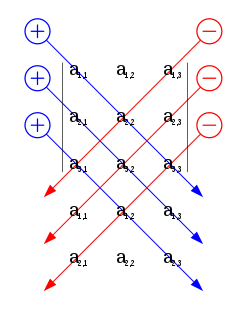
\includegraphics[scale=0.5]{Regla_de_Sarrus.png}
    \caption{Regla de Sarrus}
    \label{sarrus}
\end{figure}


Esta regla intenta emular el caso de orden dos, donde cada sumando es el producto de las diagonales, donde el signo del sumando depende de la direcci\'on de la fecha.

\begin{ejem}
Calcule el determinante de $A = \begin{pmatrix} 5 & -3 & 2 \\ 1 & 0 & 2 \\ 2 & -1 & 3 \end{pmatrix}$
\end{ejem}


\begin{ejem}
Calcule el determinante de $A = \begin{pmatrix} 2 & -3 & 5 \\ 1 & 0 & 4 \\ 3 & -3 & 9 \end{pmatrix}$
\end{ejem}

La siguiente definici\'on nos permitir\'a calcular determinantes de orden superior.
\begin{defin}
Sea $A$ una matriz de $n \times n$. La matriz $M_{ij}$ de $(n-1) \times (n-1)$ que se obtiene de $A$ eliminando la fila $i$ y la columna $j$ se llama el menor $ij$ de $A$.

Sea $A$ una matriz de $n \times n$. El cofactor $ij$ de $A$, denotado por $A_{ij}$ está dado por $A_{ij} = (-1)^{i+j}|M_{ij}|$.
\end{defin}

\begin{ejer}
\begin{enumerate}
    \item Sea $A = \begin{pmatrix} 2 & -1 & 4 \\ 0 & 1 & 5 \\ 6 & 3 & -4 \end{pmatrix}$, calcule $M_{13}$ y $M_{32}$.
    \item Sea $A = \begin{pmatrix} 1 & -3 & 5 & 6 \\ 2 & 4 & 0 & 3 \\ 1 & 5 & 9 & -2 \\ 4 & 0 & 2 & 7 \end{pmatrix}$. Calcule $A_{32}$.
\end{enumerate}
\end{ejer}


\begin{defin}
Sea $A$ una \textbf{matriz de orden $n$}. Entonces el \textbf{determinante de $A$}, denotado por $\det A$ o $|A|$
\begin{align*}
    \det: \M_{n}(K)&\to K\\
    A & \mapsto \det(A)
\end{align*}
y está dado por 
\[\det A = a_{11}A_{11}+a_{12}A_{12}+a_{13}A_{13} + \dots + a_{1n}A_{1n}.\]
\end{defin}

\begin{ejer}
Calcule el determinante de $A$
$$A = \begin{pmatrix} 2 & -3 & 0 & 1 \\ 5 & 4 & 2 & 0 \\ 1 & -1 & 0 & 3 \\ -2 & 1 & 0 & 0 \end{pmatrix}.$$
\end{ejer}





\begin{rec}
Una matriz cuadrada se denomina triangular superior si todas sus componentes abajo de la diagonal son cero. Es una matriz triangular inferior si todas sus componentes arriba de la diagonal son cero. Una matriz se denomina diagonal si todos los elementos que no se encuentran sobre la diagonal son cero.
\end{rec}

\begin{ejem}

$A = \begin{pmatrix} 2 & 1 & 7 \\ 0 & 2 & -5 \\ 0 & 0 & 1 \end{pmatrix}$; $B = \begin{pmatrix} 5 & 0 & 0 \\ 2 & 3 & 0 \\ -1 & 2 & 4 \end{pmatrix}$; $C = \begin{pmatrix} 2 & 0 & 0 \\ 0 & -7 & 0 \\ 0 & 0 & -4 \end{pmatrix}$
\end{ejem}






\begin{thm}
\begin{enumerate}
    \item Sea $A$ una matriz de $n \times n$ triangular superior o inferior. Entonces $\det A = a_{11}a_{22}a_{33} \cdots a_{nn}$.
    \item Sea $T$ una matriz triangular superior. Entonces $T$ es invertible si y solo si $\det T \not= 0$.
    \item Sean $A$ y $B$ dos matrices de orden $n$. Entonces $\det AB = (\det A) (\det B)$.
    \item $\det A^{t} = \det A$.
    \item Si cualquier fila o columna de $A$ es un vector cero, entonces $\det A = 0$.
    \item Si la fila $i$ o columna $j$ de $A$ se multiplica por un escalar $c$, entonces $\det A$ se multiplica por $c$.
\end{enumerate}
\end{thm}

\begin{ejem}
\begin{enumerate}
    \item $\begin{vmatrix} 2 & 1 & 7 \\ 0 & 2 & -5 \\ 0 & 0 & 1 \end{vmatrix} = (2)(2)(1) = 4$.
    \item Sean $A = \begin{pmatrix} 1 & -1 & 2 \\ 3 & 1 & 4 \\ 0 & -2 & 5 \end{pmatrix}$ y $B = \begin{pmatrix} 1 & -2 & 3 \\ 0 & -1 & 4 \\ 2 & 0 & -2 \end{pmatrix}$. Entonces, $\det A = 16$, $\det B = -8$ y $AB = \begin{pmatrix} 5 & -1 & -5 \\ 11 & -7 & 5 \\ 10 & 2 & -18 \end{pmatrix}$

Luego $\det AB = -128 = 16(-8) = (\det A) (\det B)$.

    \item $\begin{vmatrix} -1 & 3 & 0 & 1 \\ 4 & 2 & 0 & 5 \\ -1 & 6 & 0 & 4 \\ 2 & 1 & 0 & 1 \end{vmatrix} = 0$.
    \item Sean $A = \begin{pmatrix} 1 & -1 & 2 \\ 3 & 1 & 4 \\ 0 & -2 & 5 \end{pmatrix}$ y $C = \begin{pmatrix} 1 & -1 & 2 \\ -6 & -2 & -8 \\ 0 & -2 & 5 \end{pmatrix}$. 

Entonces $\det A = 16$ y $\det C = -32 = -2 \det A$
\end{enumerate}
\end{ejem}

\begin{rmk}
El intercambio de dos filas o columnas distintas de $A$ tiene el efecto de multiplicar $\det A$ por $-1$.
\end{rmk}
\begin{ejem}
Sean $A = \begin{pmatrix} 1 & -1 & 2 \\ 3 & 1 & 4 \\ 0 & -2 & 5 \end{pmatrix}$ y $C = \begin{pmatrix} 1 & -1 & 2 \\ 0 & -2 & 5 \\ 3 & 1 & 4 \end{pmatrix}$. 

Luego $\det A = 16$ y $\det C = -16 = - \det A$.
\end{ejem}

\begin{ejer}
\begin{enumerate}
\item Calcule el determinante de la matriz identidad de orden $n$. 
    \item Si $A$ es una matriz de orden $n$ y $k$ es un n\'umero natural. Determine $\det(A^k)$ y $\det(kA)$.
    \item Calcule el determinate de la matriz
    \[A=\begin{pmatrix} 1 & 1 & 1 \\ a & b & c \\ a^2 & b^2 & c^2 \end{pmatrix}\]
    \vspace*{0.5cm}
\end{enumerate}
\end{ejer}



\begin{rmk}
Si $A$ tiene dos filas o columnas iguales, entonces $\det A=0$.
\end{rmk}

%\begin{ejem}
%\begin{center}
%    $\begin{vmatrix} 1 & -1 & 2 \\ 5 & 7 & 3 \\ 1 & -1 & 2 \end{vmatrix} = 0$
%\end{center}
%\end{ejem}

\begin{rmk}
Si una fila o columna de $A$ es un múltiplo escalar de otra fila o columna, entonces $\det A = 0$.
\end{rmk}

\begin{ejem}
    $\begin{vmatrix} 2 & 4 & 1 & 12 \\ -1 & 1 & 0 & 3 \\ 0 & -1 & 9 & -3 \\ 7 & 3 & 6 & 9 \end{vmatrix} = 0$
\end{ejem}




\begin{ejem}
    Calcule $\begin{vmatrix} 1 & 3 & 5 & 2 \\ 0 & -1 & 3 & 4 \\ 2 & 1 & 9 & 6 \\ 3 & 2 & 4 & 8 \end{vmatrix}$
\end{ejem}

\subsection{Matriz adjunta y c\'alculo de la inversa de una matriz}
Ahora podemos generalizar lo visto para matrices de orden 2.
\begin{thm}
Si $\det A = 0$, entonces la matriz $A$ no es invertible. En caso contrario $\det A^{-1} = \frac{1}{\det A}$.
\end{thm}


\begin{defin}
Sea $A$ una matriz de $n \times n$ y sea 
$B =  \begin{pmatrix} A_{11} & A_{12} & \cdots & A_{1n} \\ A_{21} & A_{22} & \cdots & A_{2n} \\ \vdots & \vdots & & \vdots \\  A_{n1} & A_{n2} & \cdots & A_{nn} \end{pmatrix}$, la matriz de sus cofactores. 

Entonces, la adjunta de $A$, escrito $\adj A$, es la transpuesta de la matriz $B$ de $n \times n$, es decir 

\[\adj A = B^t = \begin{pmatrix} A_{11} & A_{21} & \cdots & A_{n1} \\ A_{12} & A_{22} & \cdots & A_{n2} \\ \vdots & \vdots & & \vdots \\  A_{1n} & A_{2n} & \cdots & A_{nn} \end{pmatrix}.\]
\end{defin}





\begin{ejem}
Sea $A =  \begin{pmatrix} 2 & 4 & 3 \\ 0 & 1 & -1 \\ 3 & 5 & 7 \end{pmatrix}$. Calcule $\adj(A)$
\end{ejem}




\begin{thm}
Sea $A$ una matriz de $n \times n$. Entonces $A(\adj A) = (\det A)I_n$.
\end{thm}

\begin{thm}
Sea $A$ una matriz de $n \times n$. Entonces $A$ es invertible si y solo si $\det A \not= 0$. Si $\det A \not= 0$, entonces $A^{-1} = \frac{1}{\det A}\adj A$.
\end{thm}





\begin{ejem}
Sea $A =  \begin{pmatrix} 2 & 4 & 3 \\ 0 & 1 & -1 \\ 3 & 5 & 7 \end{pmatrix}$. Calcule $A^{-1}$.
\end{ejem}



\begin{thm}
\textbf{(Resumen)} Sea $A$ una matriz de $n \times n$. Las siguientes afirmaciones son equivalentes:

\begin{enumerate}
\item
$A$ es invertible


\item
$A$ es equivalente por filas a la matriz identidad de $n \times n$.

\item
La forma escalonada por filas de $A$ tiene $n$ pivotes.

\item
$\det A \not = 0$.
\end{enumerate}
\end{thm}


\begin{subsection}{Optimizaci\'on del c\'alculo de determinante}
Una de las aplicaciones del escalonamiento es el cálculo del valor de un determinante recurriendo a las operaciones elementales.  Será preciso formalizar algunas propiedades que nos aseguren obtener el valor del determinante original mediante matrices equivalentes en las cuales el cálculo resulte sencillo o inmediato. Además, veremos que combinando apropiadamente estas propiedades con el desarrollo por cofactores se logrará gran eficacia y simplicidad en los cálculos.

\begin{thm}
Si se suma un múltiplo escalar de una fila o columna de $A$ a otra fila o columna de $A$, entonces el determinante no cambia. Es decir, el determinante el invariante por operaciones fila suma
\[|A|=|A_{F_i+\alpha F_j}|.\]
\end{thm}
Recordemos que esto \textbf{no es cierto} para la operaci\'on mulplicar por un $\alpha$, m\'as a\'un
\[|A|=\alpha^{-1}|A_{\alpha F_i}|.\]

\begin{ejer}
Obtenga el valor de $ \begin{vmatrix} x & y & z \\ 3x+3 & 3y & 3z+2 \\ x+4 & y+4 & z+4 \end{vmatrix}$ sabiendo que $ \begin{vmatrix} x & y & z \\ 3 & 0 & 2 \\ 1 & 1 & 1 \end{vmatrix}=1$.
    \vspace*{0.5cm}
\end{ejer}
Si recordamos que $|A^t| = |A|$, se nos hará evidente que, en el cálculo de un determinante, las propiedades mencionadas para las operaciones elementales entre filas serán homólogas para las operaciones elementales entre columnas. Incluso se pueden aplicar en forma combinada unas y otras.

Por lo tanto, si usamos estas tres operaciones, ya sea entre filas o entre columnas, para construir la escalonada asociada a A  que no es otra que la triangular superior equivalente , obtendremos el valor para $|A|$ multiplicando los elementos de la diagonal principal de esa triangular.


\begin{ejer}
Sea $A_\alpha=\begin{vmatrix} 2 & 1 & 4 \\ 1 & \alpha-1 & 2\\ 2 & 1 & \alpha+1  \end{vmatrix}$. Encuentre los valores de $\alpha$, de manera que la matriz $A_\alpha$ sea invertible.
\end{ejer}
Otra propiedad interesante del determinante es la siguiente
\begin{thm}
Si todos los elementos de una fila de una matriz se descomponen en la suma de dos sumandos, el
determinante de la matriz inicial es la suma de dos determinantes que tienen en una fila, respectivamente, el
primer y segundo sumando, siendo el resto de las filas iguales a las filas del determinante de la matriz inicial. Es decir,
\[\begin{vmatrix} \alpha+ a & \beta + b & \gamma + c \\ a_{12} & a_{22}  & a_{32}  \\  a_{13} & a_{23}  & a_{33} \end{vmatrix}=\begin{vmatrix} \alpha& \beta  & \gamma  \\ a_{12} & a_{22}  & a_{32}  \\  a_{13} & a_{23}  & a_{33} \end{vmatrix}+\begin{vmatrix}  a &  b &  c \\ a_{12} & a_{22}  & a_{32}  \\  a_{13} & a_{23}  & a_{33} \end{vmatrix}.\]
\end{thm}
\end{subsection}



